\chapter{Opis projektnog zadatka}
		
		\textbf{\textit{dio 1. revizije}}\\
		
		\textit{Na osnovi projektnog zadatka detaljno opisati korisničke zahtjeve. Što jasnije opisati cilj projektnog zadatka, razraditi problematiku zadatka, dodati nove aspekte problema i potencijalnih rješenja. Očekuje se minimalno 3, a poželjno 4-5 stranica opisa.	Teme koje treba dodatno razraditi u ovom poglavlju su:}
		\begin{packed_item}
			\item \textit{potencijalna korist ovog projekta}
			\item \textit{postojeća slična rješenja (istražiti i ukratko opisati razlike u odnosu na zadani zadatak). Dodajte slike koja predočavaju slična rješenja.}
			\item \textit{skup korisnika koji bi mogao biti zainteresiran za ostvareno rješenje.}
			\item \textit{mogućnost prilagodbe rješenja }
			\item \textit{opseg projektnog zadatka}
			\item \textit{moguće nadogradnje projektnog zadatka}
		\end{packed_item}
		
		\textit{Za pomoć pogledati reference navedene u poglavlju „Popis literature“, a po potrebi konzultirati sadržaj na internetu koji nudi dobre smjernice u tom pogledu.} \newline
		
		
		Cilj ovog projekta je razviti programsku podršku za stvaranje web aplikacije “Wildtrack” koja će korisnicima olakšati koordinaciju prilikom prolaženja i praćenja divljih životinja. Ovom aplikacijom želimo unaprijediti istraživačke projekte i potaknuti svijest o važnosti očuvanja divljih životinja. Planiramo stvoriti jednostavno korisničko sučelje koje će omogućiti korisnicima da zajedno doprinesu istraživanju i zaštiti divljih životinja. Ova web aplikacija će biti izuzetno korisna za praćenje kretanja životinja, analiziranje njihovih navika i migracija te pružanje važnih podataka za očuvanje njihovih prirodnih staništa.\newline
		
		Na tržištu već postoje neke slične aplikacije koje omogućavaju praćenje divljih životinja, ali Wildtrack se ističe svojom inovativnom platformom za suradnju između različitih korisničkih uloga. Neke od postojećih aplikacija su:
		
		\begin{packed_item}
			\item iNaturalist: iNaturalist je globalna mreža istraživača, znanstvenika i ljubitelja prirode koji dijele svoja opažanja divljih životinja. Korisnici mogu fotografirati i dijeliti slike biljaka i životinja, a zajednica pomaže u identifikaciji vrsta. 
			\begin{figure}[H]
				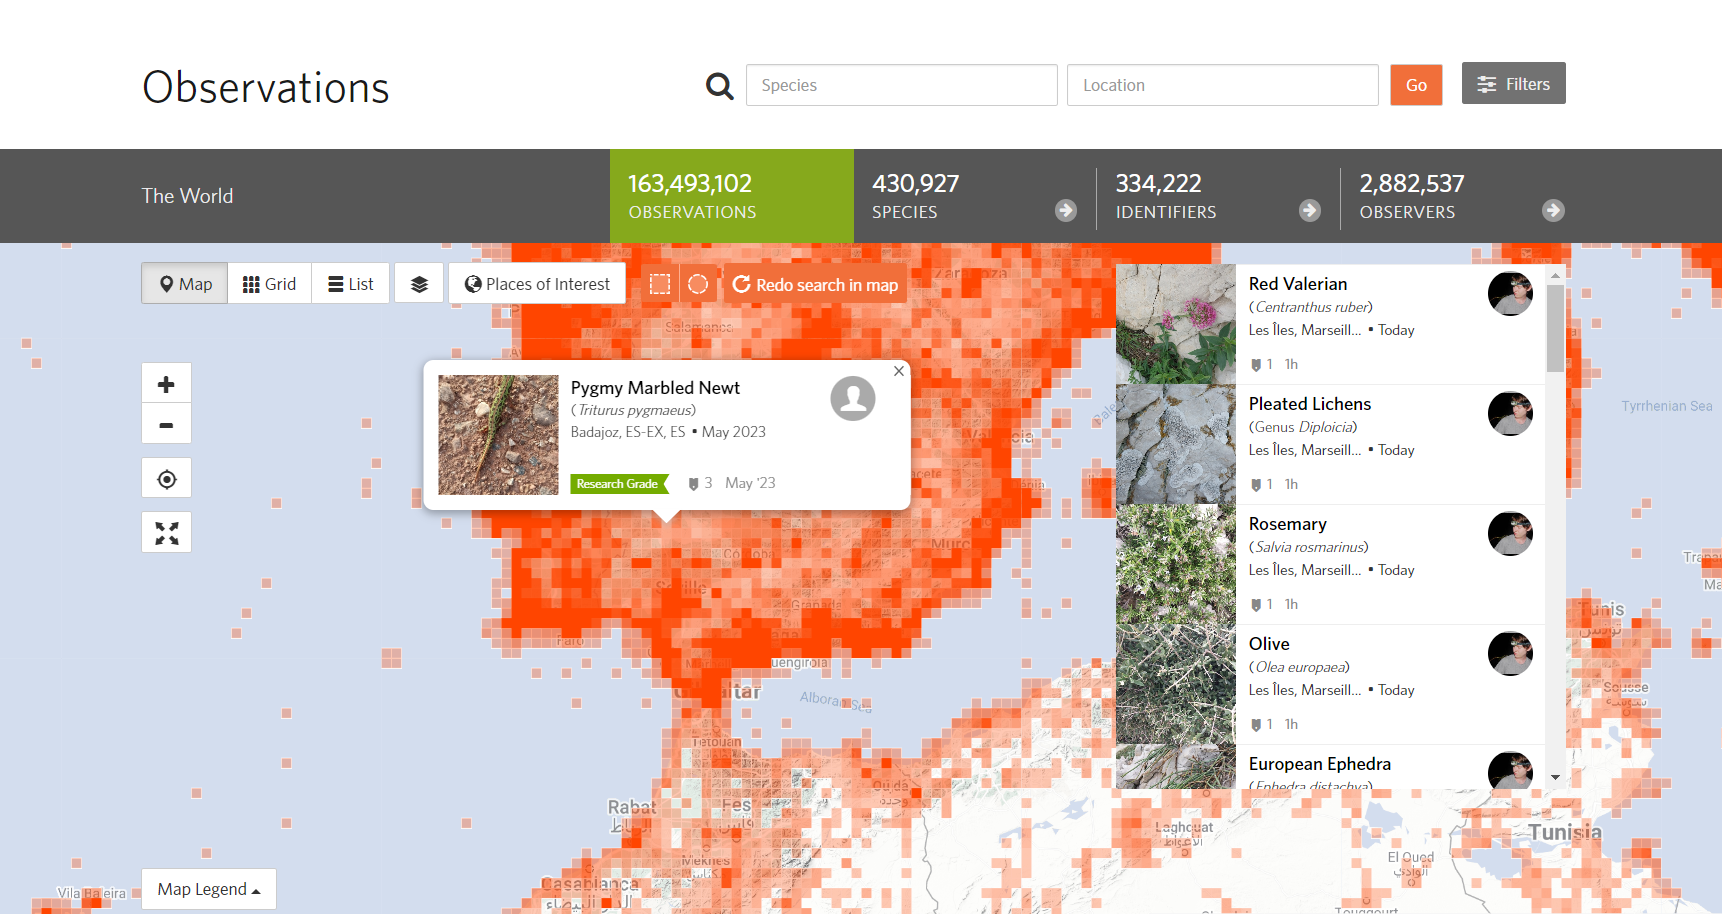
\includegraphics[width=\textwidth]{slike/inaturalist.PNG} %veličina u odnosu na širinu linije
				\caption{iNaturalist}
				\label{fig:inaturalist} %label mora biti drugaciji za svaku sliku
			\end{figure}
			
			\item eBird: eBird je aplikacija razvijena od strane Cornell Lab of Ornithology, fokusirana na ptice. Korisnici mogu bilježiti svoja opažanja o pticama te pridonositi globalnoj bazi podataka o pticama.
			\begin{figure}[H]
				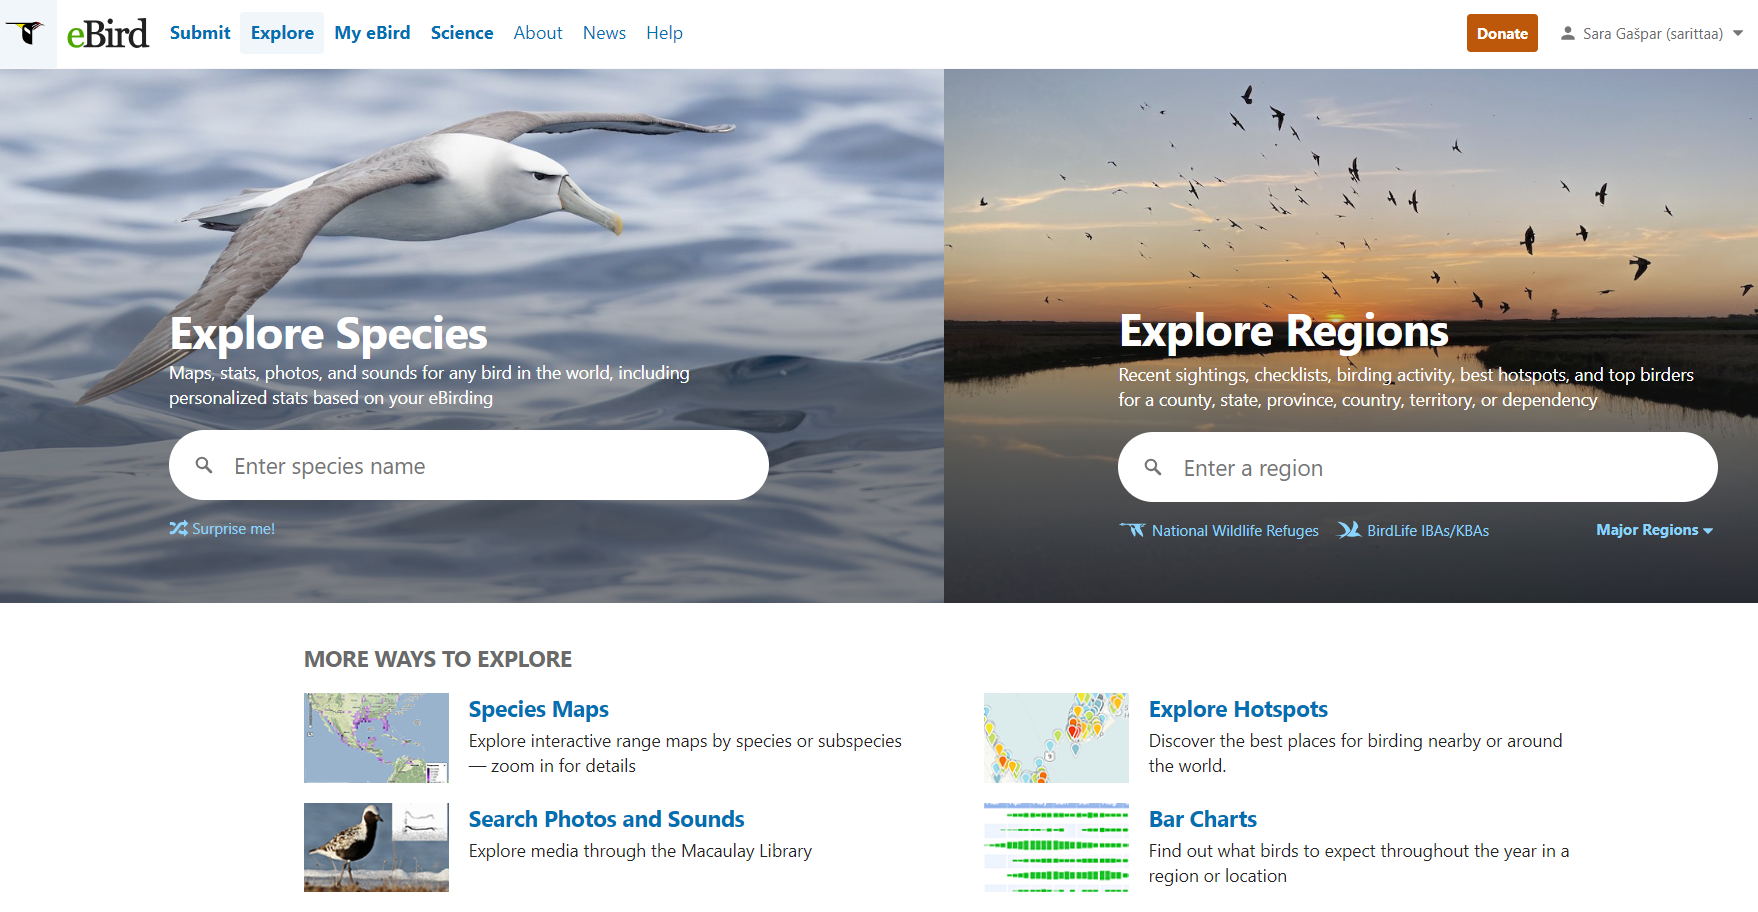
\includegraphics[width=\textwidth]{slike/ebird.PNG} %veličina u odnosu na širinu linije
				\caption{eBird}
				\label{fig:ebird} %label mora biti drugaciji za svaku sliku
			\end{figure}
			\item Movebank: Ova platforma omogućuje istraživačima da prate ponašanje divljih životinja putem GPS uređaja, odašiljača i drugih senzora, te analiziraju ove podatke u stvarnom vremenu.
			\begin{figure}[H]
				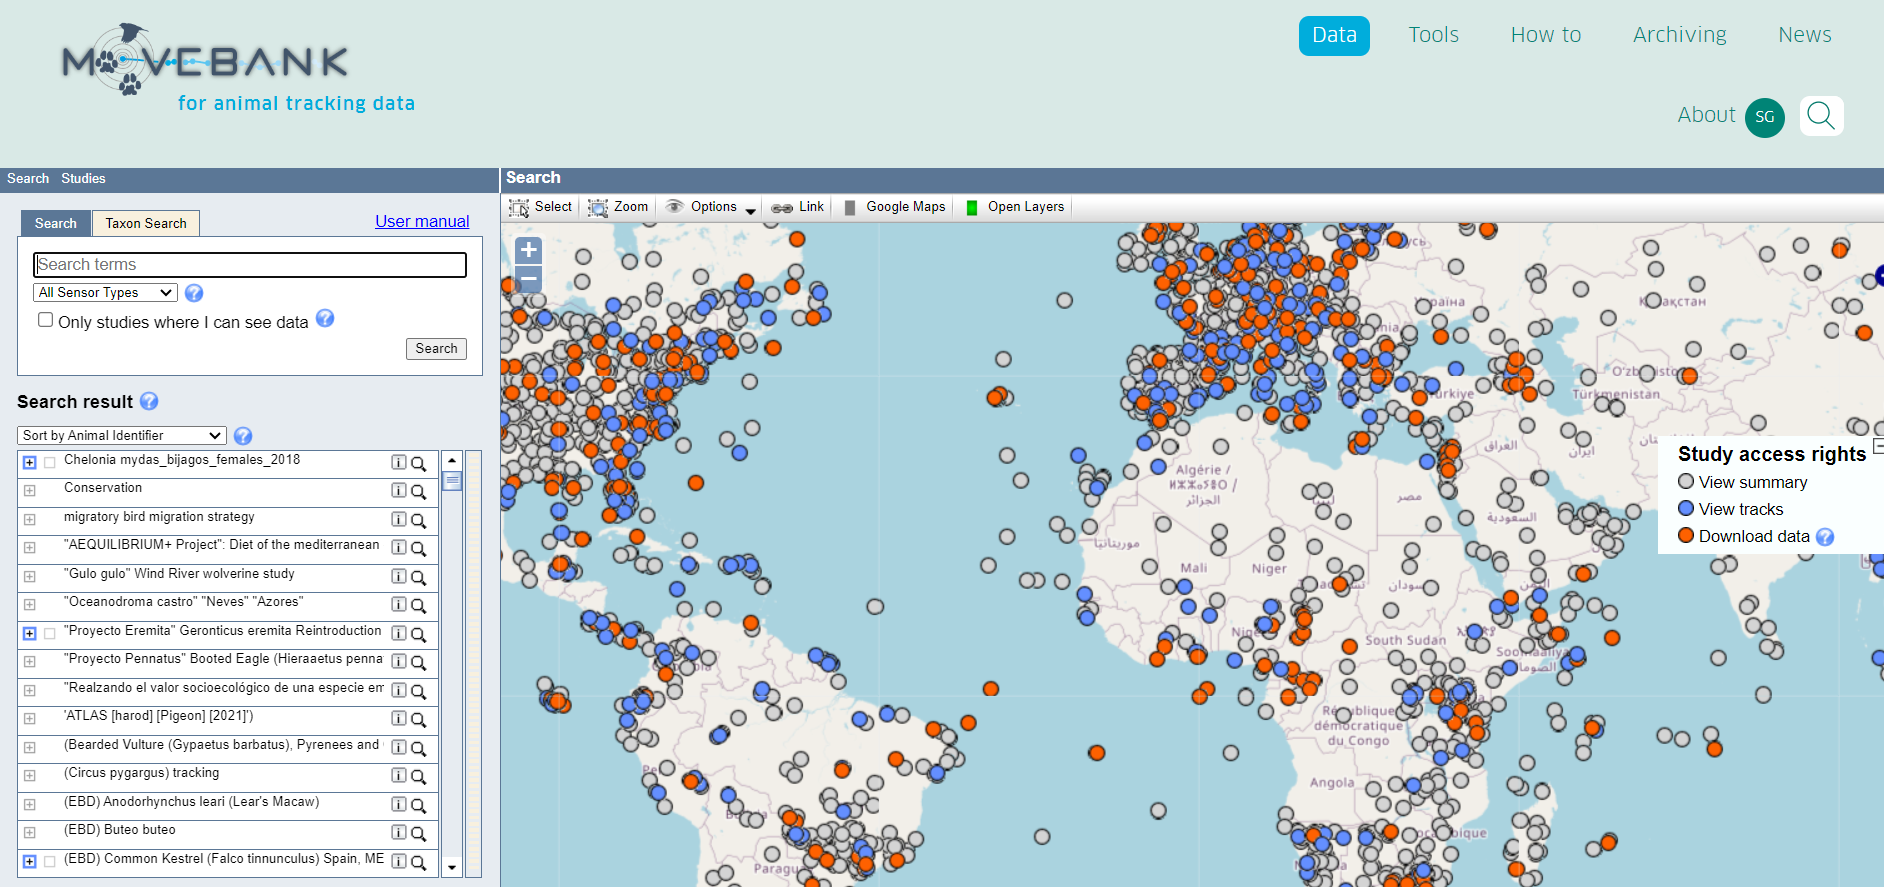
\includegraphics[width=\textwidth]{slike/movebank.PNG} %veličina u odnosu na širinu linije
				\caption{Movebank}
				\label{fig:movebank} %label mora biti drugaciji za svaku sliku
			\end{figure}
			\item Project Noah: Ova aplikacija omogućava korisnicima da dijele fotografije divljih životinja i biljaka te surađuju s globalnom zajednicom kako bi identificirali vrste.
			\begin{figure}[H]
				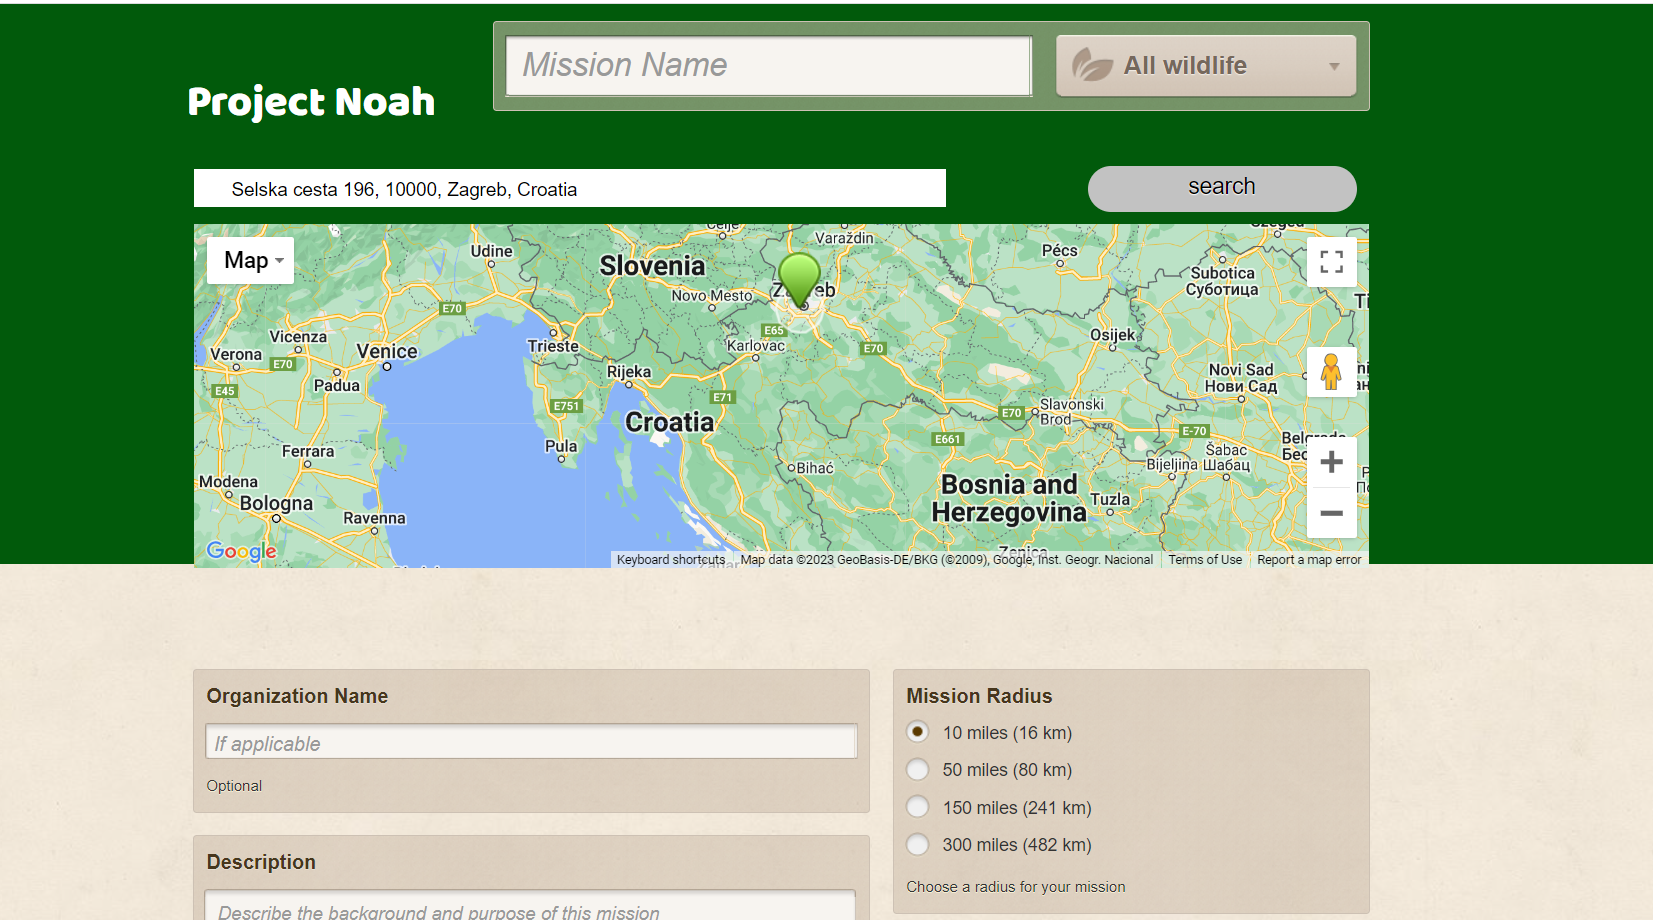
\includegraphics[width=\textwidth]{slike/projectnoah.PNG} %veličina u odnosu na širinu linije
				\caption{Project Noah}
				\label{fig:projectnoah} %label mora biti drugaciji za svaku sliku
			\end{figure}
			
		\end{packed_item}
		
		Svaka od ovih aplikacija ima svoje specifične značajke i usmjerena je na različite vrste divljih životinja ili na različite vrste istraživanja. Wildtrack bi mogao kombinirati neke od ovih značajki, kreiranje akcija poput Project Noah-a te praćenje životinja poput Movebank-a pružajući jedinstvenu platformu koja omogućava suradnju između različitih korisničkih uloga i pruža specifične alate za istraživače, voditelje postaja i terenske tragače. U nastavku ćemo detaljnije istražiti ključne značajke i prednosti ove inovativne web aplikacije.\newline
		
		Prilikom pokretanja aplikacije, neregistriranom korisniku otvara se ekran na kojem ima dvije mogućnosti: prijaviti se u sustav već postojećim računom koristeći korisničko ime i lozinku ili stvoriti novi račun registracijom. Pri stvaranju novog računa, potrebno je unijeti sljedeće podatke: korisničko ime, fotografiju, lozinku, ime, prezime te email adresu. Registrirati se može kao jedan od tri različite vrste korisnika: voditelj postaje, istraživač te tragač. Registracija se završava potvrdom preko email adrese, a istraživača i voditelja postaje dodatno treba potvrditi administrator. Tek kada je korisnik registriran i prijavljen u sustav, može iskusiti sve funkcionalnosti naše web aplikacije.\newline
		
		Praćene životinje na sebi imaju GPS uređaj koji aplikaciji odašilje svoju poziciju. O praćenim životinjama se zapisuju povijesni podaci gdje se nalazila, naziv vrste, slika i opis. Korisnicima se te informacije prikazuju na karti. \newline
		
		U aplikaciji postoje četiri različite vrste korisnika: tragač, istražitelj, voditelj postaje, te administrator. Svaka od ovih uloga ima specifične zadatke i odgovornosti. Tragači koriste GPS uređaje za praćenje životinja i obavljanje zadataka koje im dodijele istraživači. Istraživači su kreatori akcija praćenja, određuju vrste i lokacije praćenja te dodjeljuju zadatke tragačima. Voditelji postaje su odgovorni za određeno geografsko područje i organizaciju tragača unutar svoje postaje. U nastavku ćemo opisati mogućnosti i ovlasti svake od vrsta korisnika. \newline
		
		\textbf{Voditelj} postaje ima mogućnost na karti odabrati jednu od ponuđenih postaja koja obuhvaća određeni prostor i ima svoje ime, npr. postaja Lonjsko polje ili Biokovo. Kada je odabrao svoju postaju, ima mogućnost odabrati tragače svoje postaje. Osim toga, voditelj definira na koji način su njegovi tragači osposobljeni izvoditi pretraživanje. Mogu biti osposobljeni za izvođenje zadataka pješke, dronom, automobilom, cross motorom, brodom ili helikopterom. Svaka metoda pretraživanja pruža različitu vidljivost i područje pokrivanja te se na prikladan način prikazuje na karti. Voditelj također može vidjeti prikaz karte sa svojim tragačima. \newline
		
		\textbf{Istraživač} je zadužen za kreiranje novih akcija pretraživanja i praćenja s detaljima o određenim vrstama, jedinkama ili staništima za proučavanje. Svaki istraživač zadužen je samo za jednu akciju. Prilikom stvaranja akcije, istraživač voditelju stanice šalje zahtjev za tragačima. U zahtjevu treba napisati broj ljudi koji mu je potreban za akciju, te zadatke koje je potrebno obaviti. Svaka akcija ima jednog istraživača i više tragača, a odnosi se na postaju jednog ili više voditelja. Ako mu voditelj ili voditelji odobre zahtjev (imaju dovoljan broj kvalificiranih ljudi) šalju mu popis dodijeljenih tragača i tada im istraživač mora pojedinačno podijeliti konkretne zadatke. Zadatak može biti prolazak određenom rutom, dolazak do lokacije, postavljanje kamere, te postavljanje GPS uređaja za praćenje na životinje.  U slučaju da voditelj u trenutku slanja zahtjeva nema dovoljan broj odgovarajućih tragača, istraživaču će zahtjev biti odbijen, te ima mogućnost poslati novi. Istraživaču se na njegovom početnom ekranu prikazuje interaktivna karta s informacijama o pozicijama životinja, tragača i postaja. Istraživač može odabrati da se za izradu karata koriste neka od idućih informacija: povijesne pozicije svih praćenih životinja, filtrirano po vrsti ili pojedinačno po jedinki te trenutne pozicije praćenih životinja; povijesne pozicije svih tragača na nekoj akciji, filtrirano po tipu prijevoza ili pojedinačno po tragaču te trenutne pozicije tragača aktivnih na akciji. \newline
		
		\textbf{Tragač} ima ulogu praćenja životinja i obavljanja zadataka koje mu je dodijelio istraživač. Njegov početni ekran nakon prijave u sustav sadrži kartu na kojoj su mu prikazani zadaci koje treba obaviti, trenutna pozicija ostalih tragača aktivnih na istoj akciji, te trenutna pozicija praćenih životinja. Tragač na jednoj akciji ne mijenja tip prijevoza. Tragač se može maknuti s akcije završetkom svih potrebnih zadataka, a staze kojima prolazi zapisuju se u bazu. \newline
		
		\textbf{Administrator} je uloga s najvećim ovlastima i ima ju samo jedna osoba. Administrator mora potvrditi registraciju ukoliko se radi o istraživačima i voditeljima postaja. Osim toga, administrator može vidjeti popis svih registriranih korisnika i njihovih osobnih podataka te im mijenjati dodijeljena prava i osobne podatke. \newline
		
		Wildtrack također pruža mogućnost suradnje među korisnicima putem komentara i povratnih informacija. Tragači mogu ostavljati komentare o praćenju životinja, dijeliti svoja iskustva i surađivati u stvarnom vremenu. Istraživači mogu pratiti napredak svojih akcija, analizirati podatke koje prikupljaju tragači te prilagoditi strategije praćenja. Svaka akcija praćenja životinja u Wildtrack aplikaciji pridonosi bazi podataka o divljim životinjama. Ovi podaci služe istraživačima i znanstvenicima za dublje razumijevanje migracija, ponašanja i ekologije različitih vrsta. Wildtrack je više od aplikacije - to je platforma koja potiče zajednički rad i edukaciju o važnosti divljih životinja u našem ekosustavu. Ova inicijativa ima potencijal potaknuti globalnu suradnju u zaštiti prirode i očuvanju biološke raznolikosti našeg planeta. \newline
		
		
		\section{Primjeri u \LaTeX u}
		
		\textit{Ovo potpoglavlje izbrisati.}\\

		U nastavku se nalaze različiti primjeri kako koristiti osnovne funkcionalnosti \LaTeX a koje su potrebne za izradu dokumentacije. Za dodatnu pomoć obratiti se asistentu na projektu ili potražiti upute na sljedećim web sjedištima:
		\begin{itemize}
			\item Upute za izradu diplomskog rada u \LaTeX u - \url{https://www.fer.unizg.hr/_download/repository/LaTeX-upute.pdf}
			\item \LaTeX\ projekt - \url{https://www.latex-project.org/help/}
			\item StackExchange za Tex - \url{https://tex.stackexchange.com/}\\
		
		\end{itemize} 	


		
		\noindent \underbar{podcrtani tekst}, \textbf{podebljani tekst}, 	\textit{nagnuti tekst}\\
		\noindent \normalsize primjer \large primjer \Large primjer \LARGE {primjer} \huge {primjer} \Huge primjer \normalsize
				
		\begin{packed_item}
			
			\item  primjer
			\item  primjer
			\item  primjer
			\item[] \begin{packed_enum}
				\item primjer
				\item[] \begin{packed_enum}
					\item[1.a] primjer
					\item[b] primjer
				\end{packed_enum}
				\item primjer
			\end{packed_enum}
			
		\end{packed_item}
		
		\noindent primjer url-a: \url{https://www.fer.unizg.hr/predmet/proinz/projekt}
		
		\noindent posebni znakovi: \# \$ \% \& \{ \} \_ 
		$|$ $<$ $>$ 
		\^{} 
		\~{} 
		$\backslash$ 
		
		
		\begin{longtblr}[
			label=none,
			entry=none
			]{
				width = \textwidth,
				colspec={|X[8,l]|X[8, l]|X[16, l]|}, 
				rowhead = 1,
			} %definicija širine tablice, širine stupaca, poravnanje i broja redaka naslova tablice
			\hline \SetCell[c=3]{c}{\textbf{naslov unutar tablice}}	 \\ \hline[3pt]
			\SetCell{LightGreen}IDKorisnik & INT	&  	Lorem ipsum dolor sit amet, consectetur adipiscing elit, sed do eiusmod  	\\ \hline
			korisnickoIme	& VARCHAR &   	\\ \hline 
			email & VARCHAR &   \\ \hline 
			ime & VARCHAR	&  		\\ \hline 
			\SetCell{LightBlue} primjer	& VARCHAR &   	\\ \hline 
		\end{longtblr}
		

		\begin{longtblr}[
				caption = {Naslov s referencom izvan tablice},
				entry = {Short Caption},
			]{
				width = \textwidth, 
				colspec = {|X[8,l]|X[8,l]|X[16,l]|}, 
				rowhead = 1,
			}
			\hline
			\SetCell{LightGreen}IDKorisnik & INT	&  	Lorem ipsum dolor sit amet, consectetur adipiscing elit, sed do eiusmod  	\\ \hline
			korisnickoIme	& VARCHAR &   	\\ \hline 
			email & VARCHAR &   \\ \hline 
			ime & VARCHAR	&  		\\ \hline 
			\SetCell{LightBlue} primjer	& VARCHAR &   	\\ \hline 
		\end{longtblr}
	


		
		
		%unos slike
		\begin{figure}[H]
			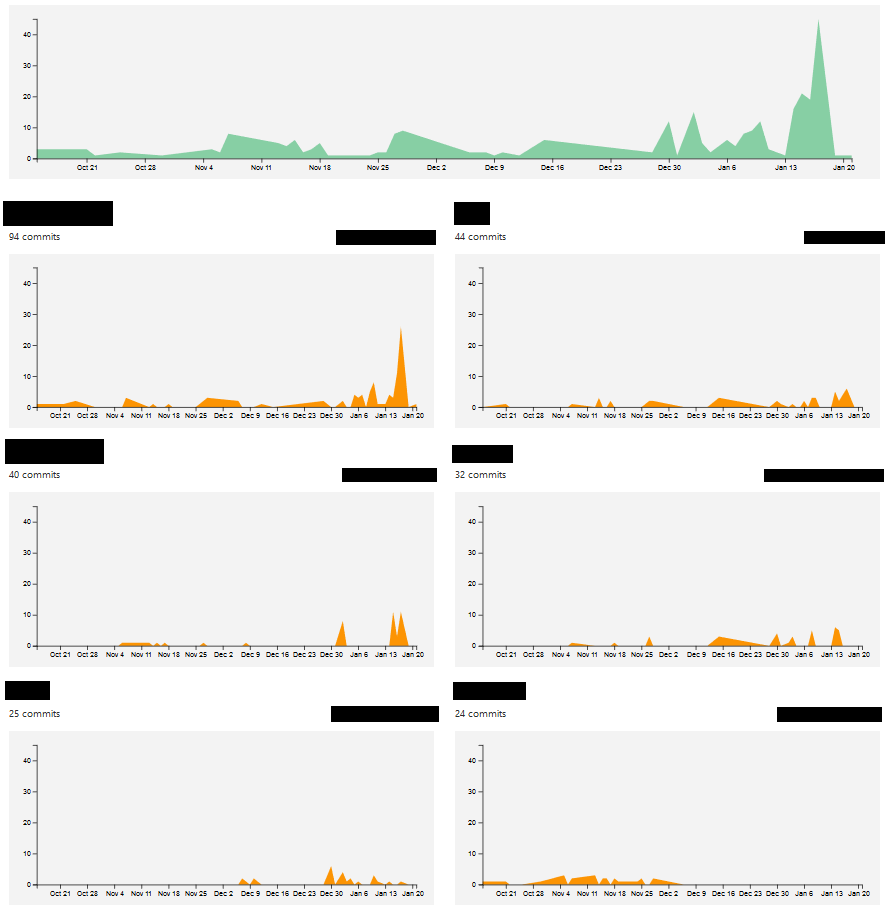
\includegraphics[scale=0.4]{slike/aktivnost.PNG} %veličina slike u odnosu na originalnu datoteku i pozicija slike
			\centering
			\caption{Primjer slike s potpisom}
			\label{fig:promjene}
		\end{figure}
		
		\begin{figure}[H]
			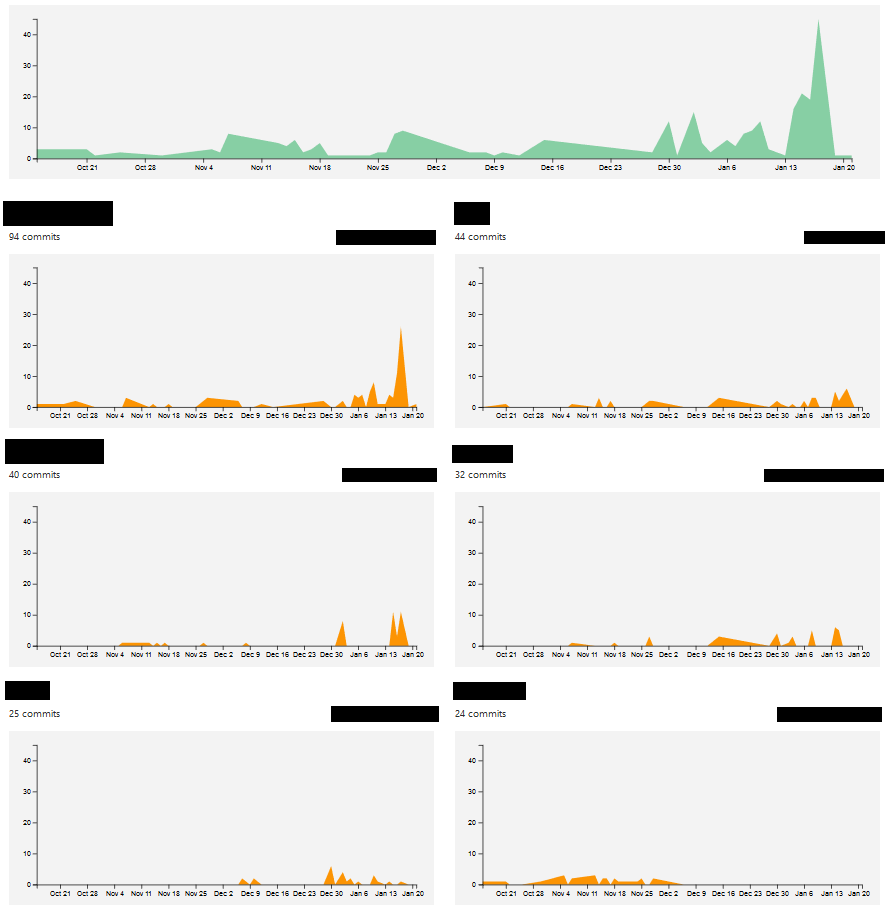
\includegraphics[width=\textwidth]{slike/aktivnost.PNG} %veličina u odnosu na širinu linije
			\caption{Primjer slike s potpisom 2}
			\label{fig:promjene2} %label mora biti drugaciji za svaku sliku
		\end{figure}
		
		Referenciranje slike \ref{fig:promjene2} u tekstu.
		
		\eject
		
	